\documentclass[a4paper,11pt]{scrartcl}

\usepackage[ngerman]{babel}
\usepackage[T1]{fontenc}
\usepackage[utf8]{inputenc}
\usepackage{microtype}
\usepackage{libertine}

% Formeln
\usepackage{amsmath}
\usepackage{mathtools}
\usepackage{booktabs}
\usepackage[version=4]{mhchem}

% Graphiken und Layout
\usepackage{float}
\usepackage{graphicx}
\usepackage{setspace}
\usepackage[separate-uncertainty=true, locale=DE]{siunitx}
\usepackage{xcolor}
\usepackage{geometry}
\geometry{left=2.5cm, right=2.5cm, top=2.5cm, bottom=2.5cm}
\usepackage[hidelinks]{hyperref}
\usepackage{microtype}







\begin{document}

\begin{titlepage}
\thispagestyle{empty}
\raggedright

\vspace*{2cm}

{\LARGE\textbf{\textsf{Praktikum Physikalische Eigenschaften von Materialien}}}

\vspace{0.5cm}

{\large Universität Augsburg\\
Wintersemester 2025/2026}

\vspace{5cm}

{\large\textbf{Versuch 7: Ferromagnetische Hystere}}

\vspace{1cm}

\begin{tabular}{ll}
\textbf{Gruppe:} & H \\
\textbf{Versuchsdatum:} & 19.02.2026 \\
\textbf{Abgabedatum:} & 31.03.2026 \\
\end{tabular}

\vspace{1.5cm}

Gemeinsames Versuchsprotokoll

\vspace{0.5cm}

Yvonne Bober \\
Antonia Scheck

\vfill

% --- Logo unten rechts ---
\begin{flushright}

\includegraphics[width=10cm]{Logo.png}
\end{flushright}

\end{titlepage}

\newpage

\tableofcontents
\thispagestyle{empty}
\cleardoublepage


\addcontentsline{toc}{section}{Abbildungsverzeichnis}
\listoffigures
\cleardoublepage 

%\addcontentsline{toc}{section}{Tabellenverzeichnis}
%\listoftables
%\cleardoublepage


\pagenumbering{arabic}
\setcounter{page}{1}
\section{Einleitung}

Magnetische Effekte begegnen in der Physik häufig zunächst in vereinfachter Form, etwa als ideales Feld einer Spule oder als lineare Beziehung zwischen Feldstärke und Magnetisierung. In realen Materialien zeigt sich jedoch ein deutlich komplexeres Verhalten. Insbesondere ferromagnetische Stoffe reagieren nicht nur auf ein aktuelles Magnetfeld, sondern behalten eine „Erinnerung“ an dessen Verlauf. Dies ist bekannt als Hysterese und ist sowohl aus physikalischer Sicht von Bedeutung als auch für zahlreiche technische Anwendungen entscheidend. \\
Ziel des vorliegenden Versuchs ist es, diese Zusammenhänge experimentell zu untersuchen. Ausgangspunkt bildet die Messung des Magnetfeldes einer stromdurchflossenen Spule, wodurch die räumliche Verteilung magnetischer Felder dargestellt wird.  \\
Darauf aufbauend wird das Verhalten ferromagnetischer Materialien im äußeren Magnetfeld betrachtet. Anhand von Hysteresekurven lässt sich nachvollziehen, wie stark die Magnetisierung vom bisherigen Feldverlauf abhängt und welche charakteristischen Kenngrößen das Materialverhalten bestimmen. Ein besonderer Fokus liegt dabei auf dem Vergleich eines Vollkerns mit einem geblätterten Eisenkern, da sich hier grundlegende Unterschiede hinsichtlich Energieverlusten und magnetischer Eigenschaften zeigen. \\
Ergänzend dazu wird die induktive Kopplung zweier Spulen genutzt, um materialabhängige Größen wie die relative Permeabilität zu bestimmen. Diese beschreibt, wie effektiv ein Material magnetische Felder verstärken und leiten kann und ist damit eine zentrale Kenngröße für technische Anwendungen. \\
Der Versuch verbindet somit grundlegende physikalische Konzepte mit praxisnahen Fragestellungen. Insbesondere wird deutlich, welche Rolle die Materialwahl für die Effizienz elektromagnetischer Systeme spielt und warum bestimmte Bauformen, wie geblätterte Kerne, in der Technik bevorzugt eingesetzt werden.


\section{Theorie} \label{sec:theorie}
\subsection{Die Solarzelle}

\newpage

\section{Versuchsbeschreibung}
Der Versuch zur Untersuchung der Solarzelle gliedert sich in drei aufeinander aufbauende Teile. Im ersten Teil wird die elektrische Kennlinie der Solarzelle aufgenommen, im zweiten Teil die spektrale Empfindlichkeit untersucht und im dritten Teil die Umwandlung und Speicherung der gewonnenen Energie anhand eines Hydro-Cars demonstriert. 

\subsection{Statische Solarzelle}
Im ersten Versuchsteils wird ein Solarzellenmodul untersucht. Dieses wird mit einer Halogenglühlampe, als künstliche Strahlungsquelle, beleuchtet und die Intenstät der einfallenden Strahlung mit einem regelbaren Transformator variiert. 
Die Solarzelle wird an einen Stromkreis mit einer Widerstandsdekade angeschlossen. Durch schrittweises Verändern des Widerstands kann der Arbeitspunkt gezielt verschoben werden. Zwei Multimeter erfassen dabei gleichzeitig Stromstärke und Spannung: Die Strommessung erfolgt in Reihe, während die Spannung parallel zur Solarzelle gemessen wird. Auf diese Weise werden für verschiedene Widerstandswerte Messpaare aufgenommen, aus denen sich die U-I-Kennlinie der Solarzelle ergibt. 
\begin{figure}[H]
    \centering
    \includegraphics[width=0.4\linewidth]{VersuchsaufbauMuster.png}
    \caption{Versuchsaufbau zur Aufnahme von U-I-Kennlinien einer Solarzelle.~\cite{leifi}} \label{fig:V1}
\end{figure}
\noindent Ergänzend werden die charakteristischen Größen Kurzschlussstrom $I_K$ und Leerlaufspannung $U_L$ bestimmt. Der Kurzschlussstrom wird durch ineinander Stecken der Kontakte und damit durch kurzschließen des Stromkreises gemessen, während für die Bestimmung der Leerlaufspannung der Stromkreis geöffnet wird, sodass kein Strom mehr fließt. 
Diese beiden Größen definieren die Randpunkte der Kennlinie und sind wesentlich für die spätere Auswertung. 
Die Messung wird für zwei unterschiedliche Strahlungsleistungen durchgeführt. Die eingestrahlte Leistung wird aus der maximalen Lampenleistung von 120 Wund der eingestellten Spannung am Transformator abgeschätzt, dessen maximale Spannung 250 V beträgt. Im Versuch wurden Messreihen bei 40\% und 80\% der maximalen Spannung aufgenommen, um den Einfluss der Beleuchtungsstärke auf das Verhalten der Solarzelle zu untersuchen. Um Messfehler zu minimieren, werden sämtliche Messungen unter möglichst vollständigem Ausschluss von Fremdlicht durchgeführt und der Dunkelstrom aufgenommen, um systematische Einflüsse berücksichtigen zu können. 

\begin{figure}[H]
    \centering
    
    \begin{minipage}[t]{0.45\linewidth}
        \centering
        \includegraphics[width=\linewidth]{Hydrocar1.jpeg}
        \caption{Versuchsaufbau der Elektrolyse des Hydro-Cars mittels Solarstrom.}
    \end{minipage}
    \hspace{0.05\linewidth}
    \begin{minipage}[t]{0.45\linewidth}
        \centering
        \includegraphics[width=\linewidth]{Hydrocar2.jpeg}
        \caption{Hydro-Car mit angeschlossener Brennstoffzelle.}
    \end{minipage}
    
\end{figure}
\newpage

\section{Auswertung und Diskussion}
\subsection{Kennliniender statischen Solarzelle}\label{sec:Aufgabe1}

\subsection{Hysteresekurve}\label{sec:Aufgabe2}
teresekurve des Vollkerns durch graphische Auswertung der Messdaten.} \label{fig:Hysteresekurve}

\begin{figure}[H]
    \centering
    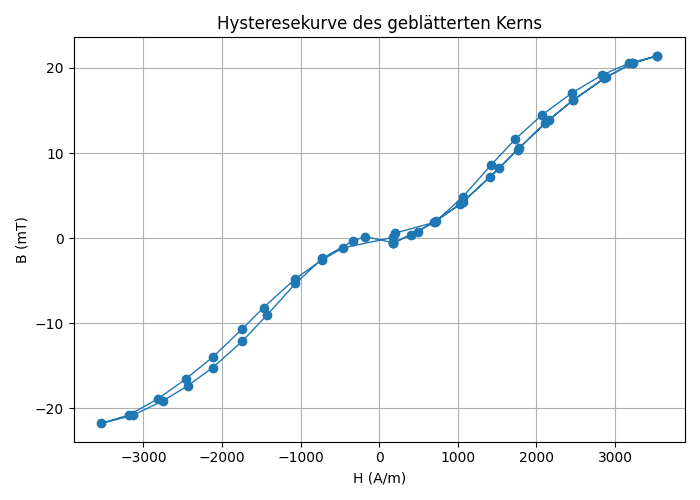
\includegraphics[width=0.4\linewidth]{Hysteresekurve-geschichteter Kern.png}
    \caption{Hysteresekurve des geblätterten Kerns durch graphische Auswertung der Messdaten.} \label{fig:HysteresekurveGeblaettert}
\end{figure}

\begin{figure}[H]
    \centering
    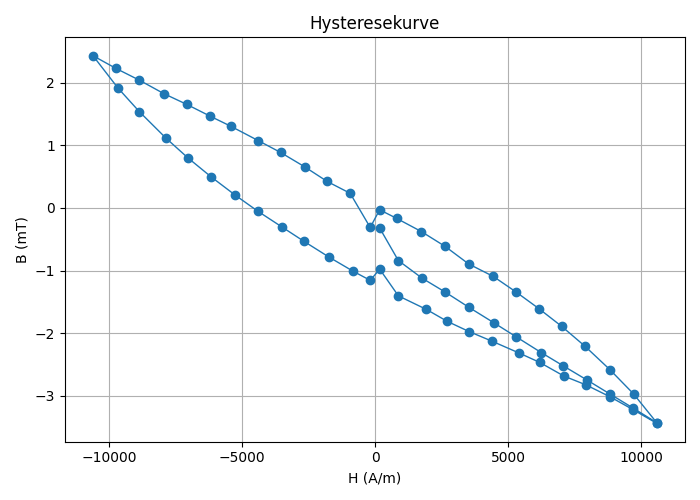
\includegraphics[width=0.4\linewidth]{Hysteresekurve-Vollkern.png}
    \caption{Hysteresekurve des Vollkerns durch graphische Auswertung der Messdaten.} \label{fig:HysteresekurveVollkern}
\end{figure}
\subsection{Untersuchung der spektralen Empfindlichkeit}\label{sec:Aufgabe3}

\newpage
\subsection{Zusammenfassung}
Im Rahmen dieses Versuchs wurde die 
\section{Anhang}
\subsection*{Laborbuch}

\begin{figure}[H]
\centering
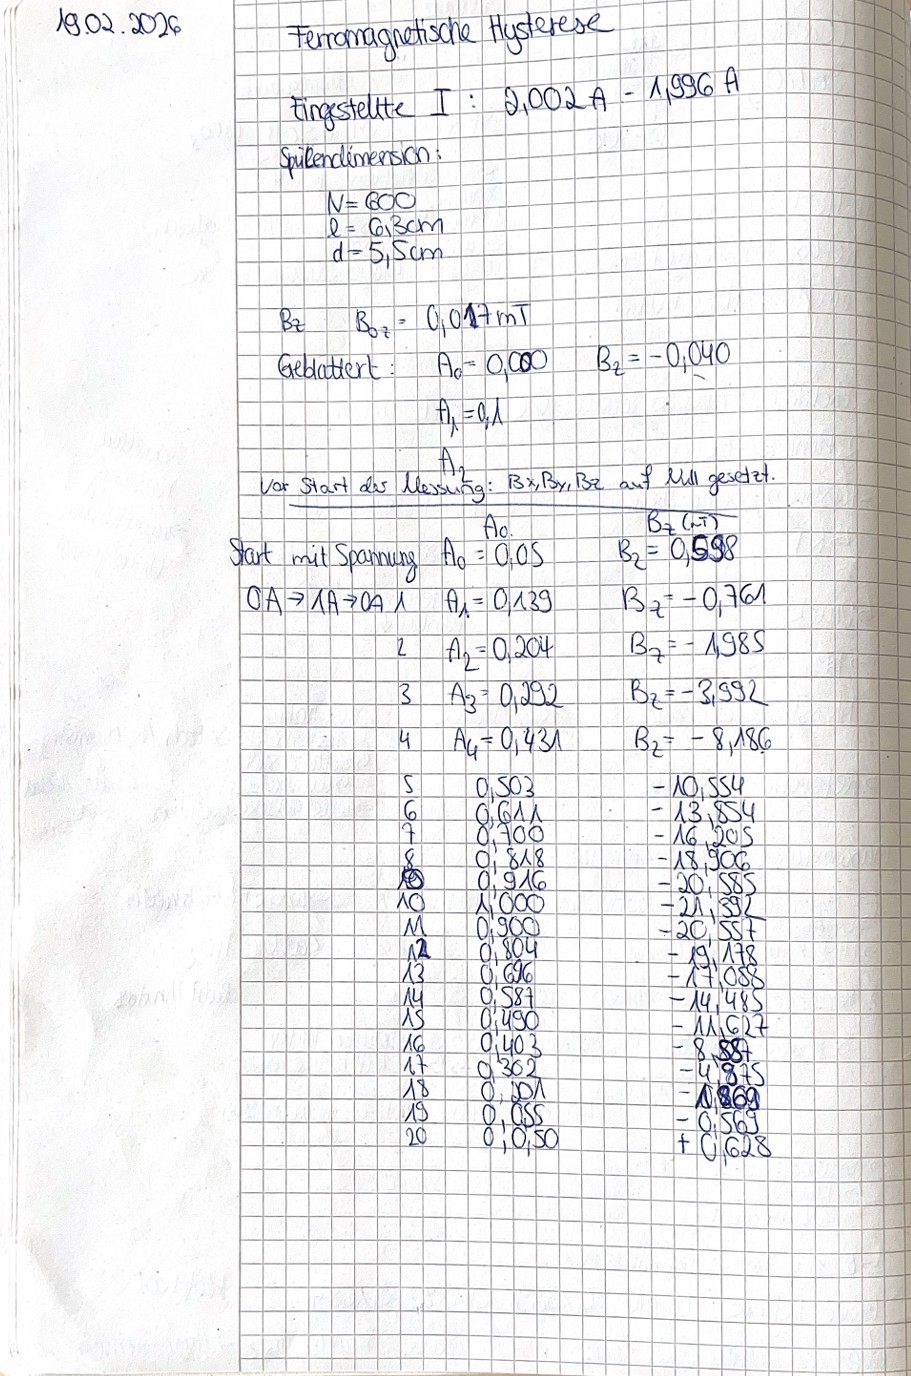
\includegraphics[width=0.8\linewidth]{heft1.png}
\caption{Laborbuch Seite 1 vom Versuch am 04.03.2026.}
\end{figure}

\begin{figure}[H]
\centering
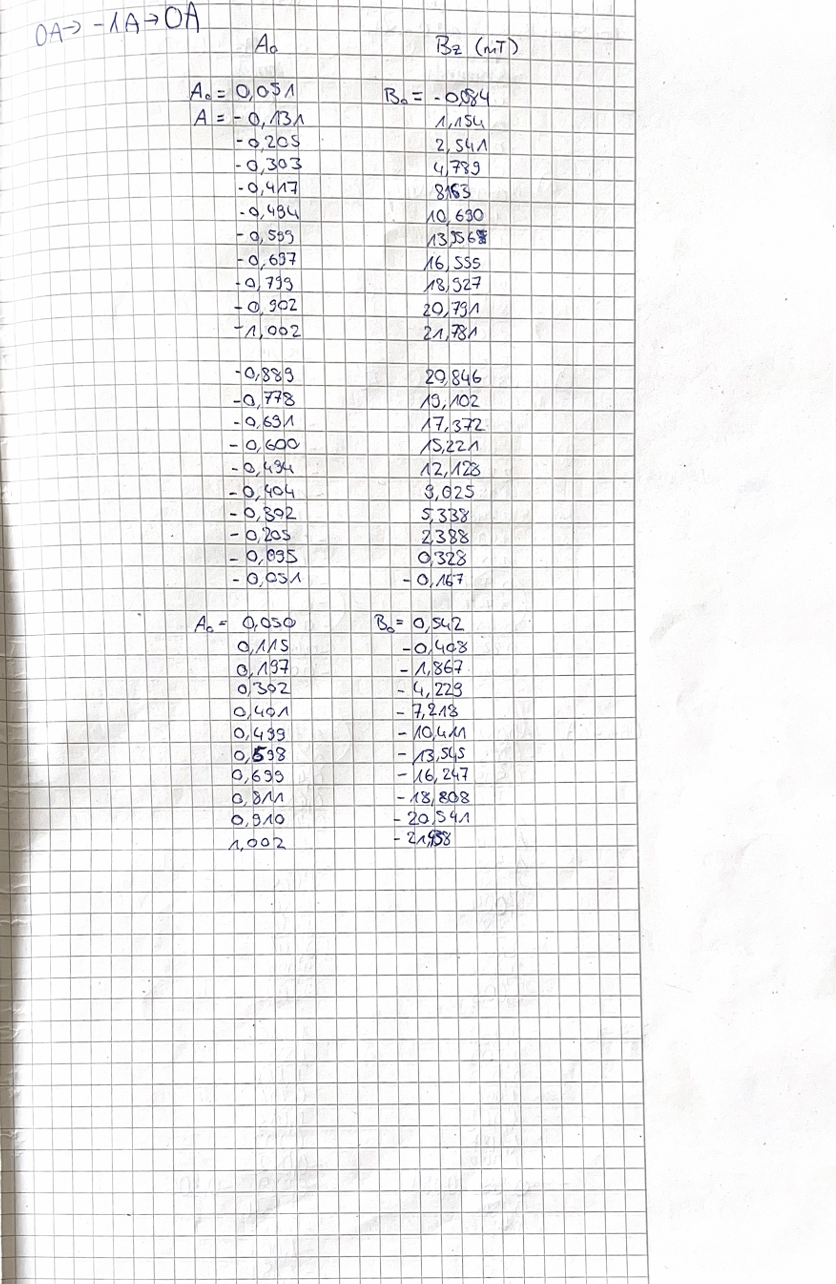
\includegraphics[width=0.8\linewidth]{heft2.png}
\caption{Laborbuch Seite 2 vom Versuch am 04.03.2026.}
\end{figure}

\begin{figure}[H]
\centering
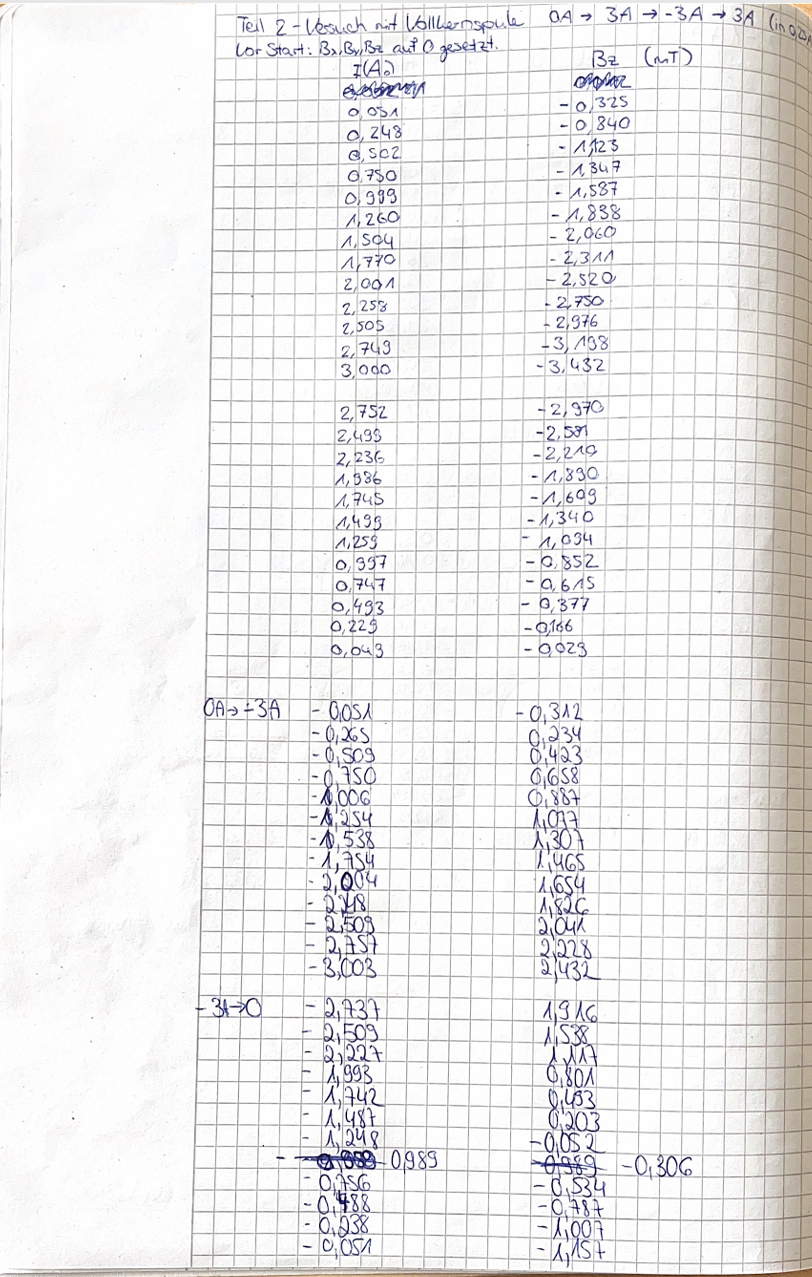
\includegraphics[width=0.8\linewidth]{heft3.png}
\caption{Laborbuch Seite 3 vom Versuch am 04.03.2026.}
\end{figure}


\newpage

\cleardoublepage
\phantomsection
\addcontentsline{toc}{section}{Literatur}
\bibliographystyle{unsrt}
\bibliography{Literatur}


\end{document}